\documentclass[aspectratio=169,11pt]{beamer}

\def\courseTitle{Industrial Security (Bachelor)}
\def\courseSubtitle{Section 02 -- ICS and SCADA Fundamentals}
\def\sectionNumber{02}
\def\sectionTitle{ICS and SCADA Fundamentals}

% =====================================================================
% Industrial Security lecture series -- modern Beamer preamble.
%
% Each slide deck must define the following BEFORE \input{}-ing this:
%   \def\courseTitle{...}        e.g. Industrial Security (Bachelor)
%   \def\courseSubtitle{...}     e.g. Section 3 -- Network Architecture
%   \def\sectionNumber{...}      e.g. 03
%   \def\sectionTitle{...}       e.g. Industrial Network Architectures
%
% Optional:
%   \def\courseAuthor{...}       defaults to "Lecture Notes"
%   \def\courseInstitute{...}    defaults to "Department of Computer Science"
%   \def\companyLogo{...}        path to a logo image (PDF/PNG/JPG).
%
% Callout macros (use anywhere inside a frame):
%   \begin{notebox}{title}      ... \end{notebox}
%   \begin{importantbox}{title} ... \end{importantbox}
%   \begin{warningbox}{title}   ... \end{warningbox}
%   \begin{tipbox}{title}       ... \end{tipbox}
%   \begin{defbox}{title}       ... \end{defbox}
%   \begin{takeawaybox}{title}  ... \end{takeawaybox}
%   \begin{quotebox}            ... \end{quotebox}
% =====================================================================

% --- Speaker-notes mode (toggled by Makefile via -usepretex) ----------
% When notesmode=1, build a side-by-side slide+notes PDF for the
% lecturer. When unset/0, build the clean slides-only PDF.
\providecommand{\notesmode}{0}
\ifnum\notesmode=1
  \usepackage{pgfpages}
  \setbeameroption{show notes on second screen=right}
  \setbeamerfont{note page}{size=\small}
\fi

\usepackage[utf8]{inputenc}
\usepackage[T1]{fontenc}
\usepackage[english]{babel}
% Modern type pair: IBM Plex Sans for text, IBM Plex Mono for code.
% Math stays in lmodern; Plex is the dominant family on every text frame.
\usepackage{plex-sans}
\usepackage{plex-mono}
\renewcommand{\familydefault}{\sfdefault}
\usepackage[activate={true,nocompatibility},final,tracking=true,kerning=true,spacing=true,factor=1100,stretch=10,shrink=10]{microtype}
\usepackage{graphicx}
\usepackage{listings}
\usepackage{xcolor}
\usepackage{colortbl}
\usepackage{tikz}
\usepackage{booktabs}
\usepackage{array}
\usepackage{hyperref}
\usepackage{amsmath}
\usepackage{amssymb}
\usepackage{tcolorbox}
\tcbuselibrary{skins, breakable, raster}
\usepackage{fontawesome5}

% =====================================================================
% Shared TikZ styles for the Industrial Security lecture series.
% Loaded by every slide deck and exercise sheet that uses TikZ.
% =====================================================================

\usetikzlibrary{
  arrows.meta,
  shapes,
  shapes.geometric,
  shapes.symbols,
  shapes.multipart,
  positioning,
  fit,
  calc,
  backgrounds,
  decorations.pathmorphing,
  decorations.pathreplacing,
  decorations.text,
  patterns,
  matrix,
  shadows
}

% --- colour palette --------------------------------------------------
\definecolor{isOT}{HTML}{1F4E79}     % OT (deep blue)
\definecolor{isIT}{HTML}{6F2DA8}     % IT (purple)
\definecolor{isSafety}{HTML}{C00000} % safety red
\definecolor{isNet}{HTML}{2E7D32}    % network green
\definecolor{isAttack}{HTML}{B23A48} % attack red
\definecolor{isAccent}{HTML}{E08E0B} % amber
\definecolor{isMute}{HTML}{6B6B6B}   % grey
\definecolor{isLight}{HTML}{EDF2F8}  % light background
\definecolor{isPLC}{HTML}{2C5282}
\definecolor{isHMI}{HTML}{2F855A}
\definecolor{isSCADA}{HTML}{6B46C1}

% --- generic node styles --------------------------------------------
\tikzset{
  isnode/.style={
    draw, rounded corners=2pt, minimum height=8mm, minimum width=18mm,
    font=\small, align=center, thick
  },
  isbox/.style={isnode, fill=isLight},
  plc/.style={isnode, fill=isPLC!15, draw=isPLC, thick},
  hmi/.style={isnode, fill=isHMI!15, draw=isHMI, thick},
  scada/.style={isnode, fill=isSCADA!15, draw=isSCADA, thick},
  sensor/.style={isnode, fill=isNet!10, draw=isNet, minimum height=6mm, minimum width=14mm, font=\scriptsize},
  actuator/.style={isnode, fill=isAccent!15, draw=isAccent, minimum height=6mm, minimum width=14mm, font=\scriptsize},
  firewall/.style={isnode, fill=isAttack!15, draw=isAttack, thick},
  server/.style={isnode, fill=isMute!15, draw=isMute!80, thick},
  switch/.style={isnode, fill=isLight, draw=black!60, minimum height=6mm, minimum width=14mm, font=\scriptsize},
  workstation/.style={isnode, fill=white, draw=isOT, thick},
  attacker/.style={isnode, fill=isAttack!20, draw=isAttack, thick, font=\small\bfseries},
  inetnode/.style={draw, ellipse, minimum width=24mm, minimum height=10mm, font=\scriptsize, fill=isLight, thick},
  process/.style={isnode, fill=isOT!15, draw=isOT, thick, minimum width=24mm},
  zone/.style={
    draw, rounded corners=4pt, thick, dashed, inner sep=4mm
  },
  conduit/.style={-{Stealth[length=2.5mm]}, thick, isNet!80!black},
  attack/.style={-{Stealth[length=2.5mm]}, thick, isAttack, dashed},
  flow/.style={-{Stealth[length=2.5mm]}, thick, isOT!70!black},
  netline/.style={thick, black!60},
  axisline/.style={-{Stealth[length=2mm]}, thick, black!70},
  tag/.style={font=\scriptsize\itshape, fill=white, inner sep=1pt},
  level/.style={
    draw, fill=isLight, minimum width=0.85\linewidth, minimum height=8mm,
    font=\small, anchor=west
  },
  brace/.style={decorate, decoration={brace, amplitude=4pt, raise=2pt}},
  legendbox/.style={draw, rounded corners=2pt, fill=isLight, inner sep=2mm, font=\scriptsize, align=left}
}

% --- handy macros ----------------------------------------------------
% \plcicon, \hmiicon etc as simple labelled boxes; useful inline.
\newcommand{\plcicon}[1][PLC]{\tikz[baseline=-0.6ex]{\node[plc, minimum width=10mm, minimum height=5mm, font=\scriptsize, inner sep=1pt]{#1};}}
\newcommand{\hmiicon}[1][HMI]{\tikz[baseline=-0.6ex]{\node[hmi, minimum width=10mm, minimum height=5mm, font=\scriptsize, inner sep=1pt]{#1};}}
\newcommand{\fwicon}[1][FW]{\tikz[baseline=-0.6ex]{\node[firewall, minimum width=10mm, minimum height=5mm, font=\scriptsize, inner sep=1pt]{#1};}}


\graphicspath{{.}{../../../template/}}

% --- defaults --------------------------------------------------------
\providecommand{\courseAuthor}{Lecture Notes}
\providecommand{\courseInstitute}{Department of Computer Science}
\providecommand{\companyLogo}{logo}

% --- modern palette --------------------------------------------------
\definecolor{slideAccent}{HTML}{1F4E79}       % primary navy
\definecolor{slideSecondary}{HTML}{E08E0B}    % amber accent

% --- Corporate branding overrides ------------------------------------
% A user-editable `branding.tex` at the repo root can override the
% logo path, author/institute lines, and brand colours. If the file is
% missing the built-in defaults above stay in effect.
\IfFileExists{../../../branding.tex}{% =====================================================================
% Corporate / institutional branding -- single file to customise the
% look of the entire course (slides, notes, exercises, labs).
%
% HOW TO REBRAND IN UNDER A MINUTE:
%   1. Replace `branding/logo.pdf` with your own logo
%      (PDF preferred; PNG and JPG also work -- name it `logo.<ext>`).
%   2. (Optional) change the two colours below to your brand palette.
%   3. (Optional) override the author/institute lines below.
%   4. Re-run `make` at the repo root. That's it.
%
% Everything in this file has sensible defaults; you can delete a line
% to fall back to the built-in defaults, or comment it out.
%
% This file is loaded automatically by the slides, exercise, and lab
% preambles -- you never need to \input it manually.
% =====================================================================

% --- Logo --------------------------------------------------------------
% Path is resolved from each leaf-build directory; the default points at
% the shared `branding/` folder at the repo root. If you put your logo
% somewhere else, set the full or relative path here (without extension):
\renewcommand{\companyLogo}{../../../branding/logo}

% --- Author / institute (appears on the title page footer) ------------
\renewcommand{\courseAuthor}{}
\renewcommand{\courseInstitute}{}

% --- Brand colours ----------------------------------------------------
% slideAccent      = primary brand colour (title bands, accent rule)
% slideSecondary   = secondary brand colour (section badge, highlight)
% Both use HTML hex codes. Keep enough contrast against white text.
\definecolor{slideAccent}{HTML}{00205B}      % deep navy
\definecolor{slideSecondary}{HTML}{00A0DC}   % light blue accent
}{}
\definecolor{slideTitle}{HTML}{0F2A44}        % near-black navy
\definecolor{slideMuted}{HTML}{6B6B6B}
\definecolor{slideBg}{HTML}{FFFFFF}
\definecolor{slidePanel}{HTML}{F4F7FB}
\definecolor{slideRule}{HTML}{D6DEE8}

% Callout colours
\definecolor{calNote}{HTML}{1F4E79}
\definecolor{calImportant}{HTML}{B23A48}
\definecolor{calWarning}{HTML}{C77700}
\definecolor{calTip}{HTML}{2E7D32}
\definecolor{calDef}{HTML}{6B46C1}
\definecolor{calTake}{HTML}{0F2A44}

% --- beamer theme ---------------------------------------------------
\useinnertheme{rectangles}
\usefonttheme{professionalfonts}

\setbeamertemplate{navigation symbols}{}
\setbeamertemplate{itemize items}[circle]
\setbeamertemplate{enumerate items}[default]
\setbeamertemplate{section in toc}[ball numbered]
\setbeamercolor{section in toc}{fg=slideTitle}

% Colours
\setbeamercolor{normal text}{fg=slideTitle, bg=slideBg}
\setbeamercolor{title}{fg=slideAccent}
\setbeamercolor{subtitle}{fg=slideMuted}
\setbeamercolor{frametitle}{fg=slideAccent}
\setbeamercolor{structure}{fg=slideAccent}
\setbeamercolor{itemize item}{fg=slideAccent}
\setbeamercolor{itemize subitem}{fg=slideSecondary}
\setbeamercolor{block title}{fg=white, bg=slideAccent}
\setbeamercolor{block body}{fg=slideTitle, bg=slidePanel}
\setbeamercolor{alerted text}{fg=slideSecondary}

% Fonts
\setbeamerfont{title}{series=\bfseries, size=\Large}
\setbeamerfont{subtitle}{series=\mdseries, size=\normalsize}
\setbeamerfont{frametitle}{series=\bfseries, size=\large}
\setbeamerfont{block title}{series=\bfseries, size=\normalsize}
\setbeamerfont{footline}{size=\tiny}

% --- frametitle: title bar + accent underline + section badge -------
% The accent rules are wrapped in a zero-width box so they never
% contribute to the surrounding hbox width (no Overfull warnings).
\setbeamertemplate{frametitle}{%
  \nointerlineskip
  \begin{beamercolorbox}[wd=\paperwidth, ht=2.8ex, dp=1.6ex, leftskip=1.2em, rightskip=1.2em]{frametitle}%
    \usebeamerfont{frametitle}\insertframetitle%
    \hfill
    {\color{slideMuted}\small \sectionNumber}%
  \end{beamercolorbox}%
  \nointerlineskip
  \makebox[0pt][l]{\hspace*{1.2em}\textcolor{slideSecondary}{\rule{2.5em}{1pt}}\textcolor{slideAccent}{\rule{\dimexpr\paperwidth-3.7em\relax}{1pt}}}%
  \par\vskip4pt
}

% --- footer ---------------------------------------------------------
\defbeamertemplate*{footline}{is-footer}{%
  \leavevmode%
  \hbox{%
    \begin{beamercolorbox}[wd=.55\paperwidth, ht=2.4ex, dp=1ex, leftskip=1em]{author in head/foot}%
      {\color{slideMuted}\tiny \courseTitle{} \;\; $\bullet$ \;\; Section \sectionNumber{} -- \sectionTitle}%
    \end{beamercolorbox}%
    \begin{beamercolorbox}[wd=.45\paperwidth, ht=2.4ex, dp=1ex, rightskip=1em]{title in head/foot}%
      \hfill {\color{slideMuted}\tiny \insertframenumber{} / \inserttotalframenumber}%
    \end{beamercolorbox}%
  }%
  \vskip2pt
}

% --- listings -------------------------------------------------------
\definecolor{codebg}{HTML}{F4F7FB}
\definecolor{codekw}{HTML}{0F2A44}
\definecolor{codestr}{HTML}{8B3A3A}
\definecolor{codecom}{HTML}{5A7D54}

\lstset{
    backgroundcolor=\color{codebg},
    basicstyle=\ttfamily\scriptsize\color{slideTitle},
    keywordstyle=\color{codekw}\bfseries,
    stringstyle=\color{codestr},
    commentstyle=\color{codecom}\itshape,
    breaklines=true,
    frame=leftline,
    framerule=2pt,
    rulecolor=\color{slideAccent},
    numbers=left,
    numberstyle=\tiny\color{slideMuted},
    numbersep=8pt,
    showstringspaces=false,
    tabsize=2,
    captionpos=b,
    xleftmargin=0.6em
}

% --- callout boxes --------------------------------------------------
% Shared base style for all callout boxes.
% Subtle drop shadow gives the boxes a hint of elevation without distraction.
\tcbset{
  isCallout/.style={
    enhanced, breakable, sharp corners=northeast,
    arc=2pt, boxrule=0pt,
    leftrule=3pt,
    fonttitle=\bfseries\small,
    coltitle=white,
    fontupper=\small,
    left=2mm, right=2mm, top=1.5mm, bottom=1.5mm,
    drop fuzzy shadow=black!30,
    title={#1}
  }
}

\newtcolorbox{notebox}[1]{
  isCallout={#1},
  colback=calNote!8, colframe=calNote, leftrule=3pt,
  colbacktitle=calNote, attach boxed title to top left={xshift=2mm, yshift=-1.2mm},
  boxed title style={colback=calNote, arc=1pt, boxrule=0pt, left=2mm, right=2mm, top=0.5mm, bottom=0.5mm}
}

\newtcolorbox{importantbox}[1]{
  isCallout={#1},
  colback=calImportant!7, colframe=calImportant, leftrule=4pt,
  colbacktitle=calImportant, attach boxed title to top left={xshift=2mm, yshift=-1.2mm},
  boxed title style={colback=calImportant, arc=1pt, boxrule=0pt, left=2mm, right=2mm, top=0.5mm, bottom=0.5mm}
}

\newtcolorbox{warningbox}[1]{
  isCallout={#1},
  colback=calWarning!10, colframe=calWarning, leftrule=4pt,
  colbacktitle=calWarning, attach boxed title to top left={xshift=2mm, yshift=-1.2mm},
  boxed title style={colback=calWarning, arc=1pt, boxrule=0pt, left=2mm, right=2mm, top=0.5mm, bottom=0.5mm}
}

% Alias warnbox = warningbox, with an optional title (default = "Caution")
\newtcolorbox{warnbox}[1][Caution]{
  isCallout={#1},
  colback=calWarning!10, colframe=calWarning, leftrule=4pt,
  colbacktitle=calWarning, attach boxed title to top left={xshift=2mm, yshift=-1.2mm},
  boxed title style={colback=calWarning, arc=1pt, boxrule=0pt, left=2mm, right=2mm, top=0.5mm, bottom=0.5mm}
}

\newtcolorbox{tipbox}[1]{
  isCallout={#1},
  colback=calTip!8, colframe=calTip, leftrule=3pt,
  colbacktitle=calTip, attach boxed title to top left={xshift=2mm, yshift=-1.2mm},
  boxed title style={colback=calTip, arc=1pt, boxrule=0pt, left=2mm, right=2mm, top=0.5mm, bottom=0.5mm}
}

\newtcolorbox{defbox}[1]{
  isCallout={#1},
  colback=calDef!8, colframe=calDef, leftrule=3pt,
  colbacktitle=calDef, attach boxed title to top left={xshift=2mm, yshift=-1.2mm},
  boxed title style={colback=calDef, arc=1pt, boxrule=0pt, left=2mm, right=2mm, top=0.5mm, bottom=0.5mm}
}

\newtcolorbox{takeawaybox}[1]{
  enhanced, breakable, arc=3pt, boxrule=0pt,
  colback=calTake!7, colframe=calTake,
  toptitle=2mm, bottomtitle=2mm,
  fonttitle=\bfseries\normalsize, coltitle=white,
  colbacktitle=calTake,
  fontupper=\small,
  title={\faStar~Key Takeaway: #1},
  left=3mm, right=3mm, top=2mm, bottom=2mm
}

\newtcolorbox{quotebox}{
  enhanced, breakable, arc=2pt, boxrule=0pt,
  colback=slidePanel, colframe=slideMuted,
  leftrule=3pt, top=2mm, bottom=2mm, left=3mm, right=3mm,
  fontupper=\itshape\small,
}

% Convenience: inline highlight badge
\newcommand{\remembertag}{\tikz[baseline=-0.7ex]\node[fill=calImportant, text=white, font=\scriptsize\bfseries, rounded corners=2pt, inner sep=2pt]{REMEMBER};}
\newcommand{\tldr}{\tikz[baseline=-0.7ex]\node[fill=calTake, text=white, font=\scriptsize\bfseries, rounded corners=2pt, inner sep=2pt]{TL;DR};}

% Source attribution: tiny grey line, anchored bottom-left of the content area
% Usage:  \source{Symantec, \emph{W32.Stuxnet Dossier} v1.4, 2011.}
% Multiple sources:  \source{X.\ Y., 2018; Z, 2020.}
\newcommand{\source}[1]{%
  \par\nointerlineskip\vspace{0.4mm}%
  {\color{slideMuted}\fontsize{5.5}{6.5}\selectfont\textit{Source:} #1\par}%
}

% References slide: aggregate citations + further reading at the end of a section.
% Usage:  \referencesframe{ \item ... \item ... }
% The `frame` environment must be written literally in the deck, so this is a
% macro rather than a wrapper environment (beamer collects the frame body and
% trips over \newenvironment wrappers).
%
% allowframebreakstemplate=\insertcontinuationcount silences the trailing roman
% numeral when content fits on a single page.
\setbeamertemplate{frametitle continuation}[from second]
\newcommand{\referencesframe}[1]{%
  \begin{frame}[allowframebreaks]{References -- Section \sectionNumber}
    \fontsize{7.5}{9}\selectfont
    \setlength{\itemsep}{1pt}
    \begin{itemize}#1\end{itemize}
  \end{frame}%
}

% --- title page -----------------------------------------------------
\title[\courseTitle]{\courseTitle}
\subtitle{\courseSubtitle}
\author{\courseAuthor}
\institute{\courseInstitute}
\date{}

% Logo lookup: try the section directory, then the shared template/.
\newcommand{\showlogo}[1][2cm]{%
  \IfFileExists{\companyLogo.pdf}{\includegraphics[width=#1]{\companyLogo}}{%
    \IfFileExists{\companyLogo.png}{\includegraphics[width=#1]{\companyLogo}}{%
      \IfFileExists{\companyLogo.jpg}{\includegraphics[width=#1]{\companyLogo}}{%
        \IfFileExists{../../../template/\companyLogo.pdf}{\includegraphics[width=#1]{../../../template/\companyLogo}}{%
          \rule{0pt}{0pt}}}}}}

\setbeamertemplate{title page}{%
  
\begin{tikzpicture}[remember picture, overlay]
    % accent band (taller to fit wrapped titles)
    \fill[slideAccent] (current page.north west) rectangle ([yshift=-3.4cm]current page.north east);
    \fill[slideSecondary] ([yshift=-3.4cm]current page.north west) rectangle ([yshift=-3.55cm]current page.north east);
    % section badge
    \node[fill=slideSecondary, text=white, font=\bfseries\normalsize, rounded corners=3pt, inner sep=4pt, anchor=north west]
      at ([xshift=1.2cm, yshift=-0.7cm]current page.north west) {Section \sectionNumber};
    % Course title (wraps if long)
    \node[anchor=north west, text=white, font=\bfseries\Large, align=left, text width=11cm]
      at ([xshift=1.2cm, yshift=-1.5cm]current page.north west) {\courseTitle};
    % Subtitle (wraps; smaller, separated)
    \node[anchor=north west, text=white, font=\mdseries\small, align=left, text width=11cm]
      at ([xshift=1.2cm, yshift=-2.7cm]current page.north west) {\courseSubtitle};
    \node[anchor=north east] at ([xshift=-1.2cm, yshift=-1.0cm]current page.north east)
      {\showlogo[2cm]};
    \node[anchor=south west, text=slideMuted, font=\small, align=left, text width=11cm]
      at ([xshift=1.2cm, yshift=1.0cm]current page.south west)
      {\textbf{\sectionTitle}\\[2pt]\textit{\courseAuthor}\\{\scriptsize\courseInstitute}};
  \end{tikzpicture}
}

% --- helper macros --------------------------------------------------
\newcommand{\learningobjectives}[1]{%
  \begin{frame}{Learning Objectives}
    \begin{tipbox}{\faGraduationCap~By the end of this section you will be able to}
      \begin{itemize}\setlength{\itemsep}{2pt}#1\end{itemize}
    \end{tipbox}
  \end{frame}}

\newcommand{\sectionoverviewframe}{%
  \begin{frame}[plain,noframenumbering]
    \titlepage
  \end{frame}
  \begin{frame}{Outline -- Section \sectionNumber}
    \tableofcontents
  \end{frame}}

\AtBeginSection[]{%
  \begin{frame}[plain,noframenumbering]
    \begin{tikzpicture}[remember picture, overlay]
      \fill[slideAccent] (current page.north west) rectangle (current page.south east);
      \fill[slideSecondary] ([yshift=-1pt]current page.center -| current page.west)
                            rectangle ([yshift=1pt]current page.center -| current page.east);
      \node[text=white, font=\scriptsize, anchor=south west]
        at ([xshift=1.2cm, yshift=1.0cm]current page.south west)
        {Section \sectionNumber{} -- \sectionTitle};
      \node[text=slideSecondary, font=\bfseries\Huge, anchor=south]
        at ([yshift=0.4cm]current page.center)
        {\thesection};
      \node[text=white, font=\bfseries\LARGE, align=center, anchor=north, text width=12cm]
        at ([yshift=-0.6cm]current page.center)
        {\insertsection};
    \end{tikzpicture}
  \end{frame}}

\newcommand{\closingframe}{%
  \begin{frame}[plain,noframenumbering]
    \begin{tikzpicture}[remember picture, overlay]
      \fill[slideAccent] (current page.north west) rectangle (current page.south east);
      \node[text=white, font=\bfseries\Huge, anchor=center, align=center, text width=14cm]
        at ([yshift=8mm]current page.center) {End of Section \sectionNumber};
      \fill[slideSecondary] ([xshift=-1.5cm, yshift=-4mm]current page.center)
                            rectangle ([xshift=1.5cm, yshift=-6mm]current page.center);
      \node[text=white, font=\large, anchor=north, align=center, text width=14cm]
        at ([yshift=-1.2cm]current page.center) {\sectionTitle};
      \node[text=slideSecondary, font=\normalsize, anchor=south] at ([yshift=1.2cm]current page.south) {Questions and discussion};
      \node[anchor=south east] at ([xshift=-1cm, yshift=1cm]current page.south east) {\showlogo[1.5cm]};
    \end{tikzpicture}
  \end{frame}}


\begin{document}

\sectionoverviewframe

\learningobjectives{
  \item Identify the components of a typical industrial control loop.
  \item Distinguish PLC, RTU, DCS, SCADA, HMI, Historian, and SIS.
  \item Explain the scan cycle and determinism requirements of PLCs.
  \item Read a simple ladder-logic program.
  \item Recognise why Safety Instrumented Systems must remain independent.
}

\section{Control Loop and Field Devices}

\begin{frame}{Anatomy of a Control Loop}
\centering
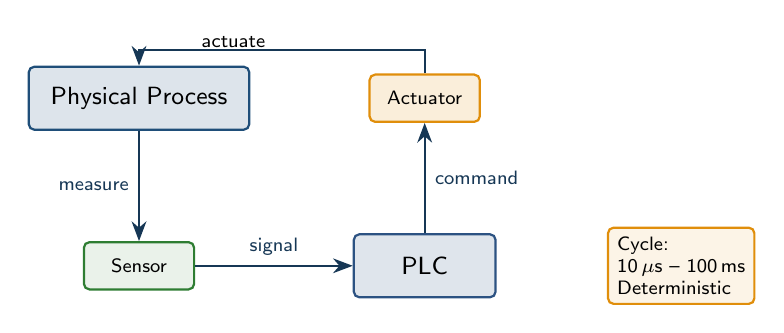
\begin{tikzpicture}[node distance=14mm]
  \node[process, minimum width=28mm, font=\small] (proc) {Physical Process};
  \node[sensor, below=of proc] (sens) {Sensor};
  \node[plc, right=20mm of sens] (plc) {PLC};
  \node[actuator, above=14mm of plc] (act) {Actuator};
  \draw[flow] (proc.south) -- (sens.north) node[midway, left, font=\scriptsize] {measure};
  \draw[flow] (sens.east) -- (plc.west) node[midway, above, font=\scriptsize] {signal};
  \draw[flow] (plc.north) -- (act.south) node[midway, right, font=\scriptsize] {command};
  \draw[flow] (act.north) -- ++(0,3mm) -| (proc.north);
  \node[font=\scriptsize, above=1mm of proc.north, xshift=12mm] {actuate};
  \node[isbox, fill=isAccent!10, draw=isAccent, right=14mm of plc, font=\scriptsize, align=left]
    {Cycle:\\10\,$\mu$s -- 100\,ms\\Deterministic};
\end{tikzpicture}
\end{frame}

\begin{frame}{Programmable Logic Controllers (PLCs)}
\begin{columns}[T,onlytextwidth]
\column{0.45\textwidth}
\small
\begin{itemize}
  \item Ruggedised industrial computer
  \item First model: Modicon 084 (1969)
  \item Replaced relay logic in plants
  \item IEC 61131-3 languages:
    \begin{itemize}\scriptsize
      \item Ladder Diagram (LD)
      \item Structured Text (ST)
      \item Function Block (FBD)
      \item Sequential Function Chart
      \item Instruction List
    \end{itemize}
\end{itemize}
{\color{slideMuted}\tiny\textit{Source:} D.\ Morley, ``History of the PLC'', Modicon, 2003 \textbar{} IEC 61131-3:2013.\par}
\column{0.55\textwidth}
\centering
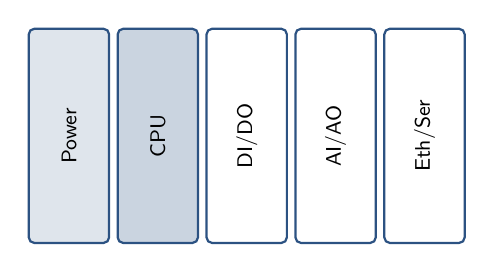
\begin{tikzpicture}[node distance=1mm, scale=0.85, transform shape]
  \node[isbox, fill=isPLC!15, draw=isPLC, minimum width=12mm, minimum height=32mm] (cpu) {\rotatebox{90}{Power}};
  \node[isbox, fill=isPLC!25, draw=isPLC, minimum width=12mm, minimum height=32mm, right=of cpu] (psu) {\rotatebox{90}{CPU}};
  \node[isbox, fill=white, draw=isPLC, minimum width=12mm, minimum height=32mm, right=of psu] (di) {\rotatebox{90}{DI/DO}};
  \node[isbox, fill=white, draw=isPLC, minimum width=12mm, minimum height=32mm, right=of di] (ai) {\rotatebox{90}{AI/AO}};
  \node[isbox, fill=white, draw=isPLC, minimum width=12mm, minimum height=32mm, right=of ai] (com) {\rotatebox{90}{Eth/Ser}};
\end{tikzpicture}
\end{columns}
\end{frame}

\begin{frame}{PLC Scan Cycle}
\centering
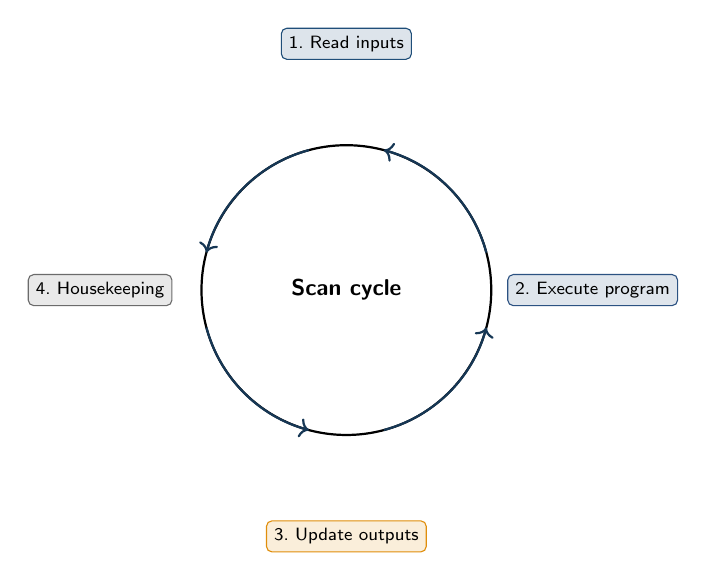
\begin{tikzpicture}[scale=0.92, transform shape]
  \def\R{2.0}
  \draw[thick] (0,0) circle (\R);
  \foreach \deg/\lbl/\col in {
    90/{1. Read inputs}/isOT,
    0/{2. Execute program}/isPLC,
    -90/{3. Update outputs}/isAccent,
    180/{4. Housekeeping}/isMute}{
    \node[fill=\col!15, draw=\col, rounded corners=2pt, font=\scriptsize, align=center, inner sep=3pt]
      at (\deg:\R+1.4) {\lbl};
  }
  \foreach \deg in {45,135,225,315}{
    \draw[->, thick, isOT!70!black] (\deg-30:\R) arc (\deg-30:\deg+30:\R);
  }
  \node[font=\small\bfseries] at (0,0) {Scan cycle};
\end{tikzpicture}
\end{frame}

\begin{frame}[fragile]{Ladder Logic --- A Motor Start/Stop}
\centering
\begin{tikzpicture}[x=8mm, y=8mm]
  % power rails
  \draw[thick] (0,3) -- (0,-2);
  \draw[thick] (12,3) -- (12,-2);
  % Rung 1: Start_Btn (NO) -- Stop_Btn (NC) -- Motor_Run coil
  \draw[thick] (0,2) -- (2,2);
  \node[font=\tiny, above=1mm] at (2.5,2) {Start};
  \draw[thick] (2,2.3) -- (2,1.7); \draw[thick] (3,2.3) -- (3,1.7);
  \draw[thick] (3,2) -- (5,2);
  \node[font=\tiny, above=1mm] at (5.5,2) {Stop (NC)};
  \draw[thick] (5,2.3) -- (5,1.7); \draw[thick] (6,2.3) -- (6,1.7);
  \draw[thick] (5,2.3) -- (6,1.7);
  \draw[thick] (6,2) -- (10,2);
  \draw[thick] (10,2) circle (4pt);
  \node[font=\tiny, above right=0mm and 1mm of {(10,2)}] {Motor\_Run};
  \draw[thick] (10.1,2) -- (12,2);
  % Rung 2: latch
  \draw[thick] (0,0) -- (2,0);
  \node[font=\tiny, above=1mm] at (2.5,0) {Motor\_Run};
  \draw[thick] (2,0.3) -- (2,-0.3); \draw[thick] (3,0.3) -- (3,-0.3);
  \draw[thick] (3,0) -- (5,0);
  % Tie rung 2 into rung 1 (parallel/seal-in)
  \draw[thick] (5,0) -- (5,2);
\end{tikzpicture}
\par\vspace{1mm}
{\footnotesize Pressing \texttt{Start} energises the coil; rung 2 latches it. \texttt{Stop} (NC) breaks both paths.}
\end{frame}

\section{Plant-Wide Architectures}

\begin{frame}{RTU vs.\ PLC vs.\ DCS}
\centering
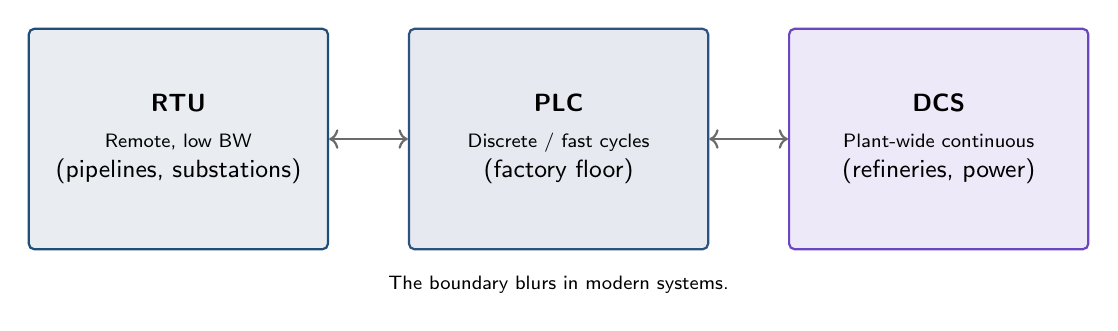
\begin{tikzpicture}[node distance=10mm]
  \node[isbox, fill=isOT!10, draw=isOT, minimum width=38mm, minimum height=28mm, align=center] (rtu)
    {\textbf{RTU}\\[2pt]\scriptsize Remote, low BW\\(pipelines, substations)};
  \node[isbox, fill=isPLC!12, draw=isPLC, minimum width=38mm, minimum height=28mm, right=of rtu, align=center] (plc)
    {\textbf{PLC}\\[2pt]\scriptsize Discrete / fast cycles\\(factory floor)};
  \node[isbox, fill=isSCADA!12, draw=isSCADA, minimum width=38mm, minimum height=28mm, right=of plc, align=center] (dcs)
    {\textbf{DCS}\\[2pt]\scriptsize Plant-wide continuous\\(refineries, power)};
  \draw[<->, thick, isMute] (rtu) -- (plc);
  \draw[<->, thick, isMute] (plc) -- (dcs);
  \node[font=\scriptsize, below=2mm of plc] {The boundary blurs in modern systems.};
\end{tikzpicture}
\end{frame}

\begin{frame}{SCADA Architecture}
\centering
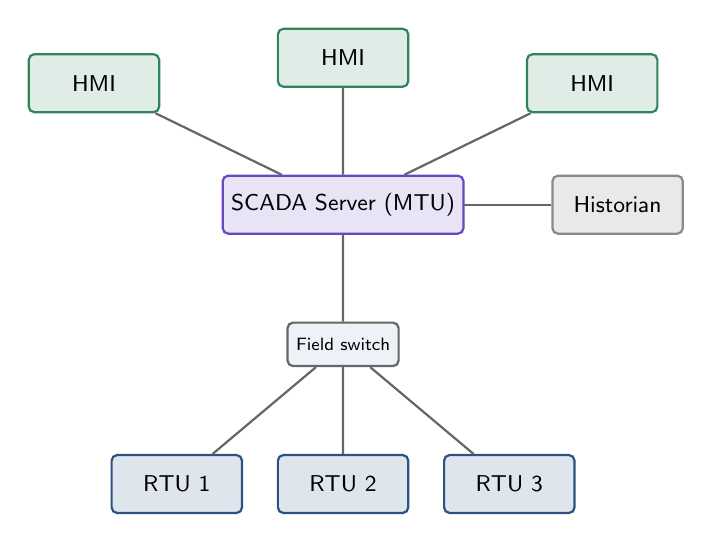
\begin{tikzpicture}[node distance=12mm, scale=0.92, transform shape]
  \node[scada] (mtu) {SCADA Server (MTU)};
  \node[hmi, above left=of mtu] (h1) {HMI};
  \node[hmi, above=of mtu] (h2) {HMI};
  \node[hmi, above right=of mtu] (h3) {HMI};
  \node[server, right=of mtu] (hist) {Historian};
  \node[switch, below=of mtu] (sw) {Field switch};
  \node[plc, below left=12mm and 6mm of sw] (p1) {RTU 1};
  \node[plc, below=12mm of sw] (p2) {RTU 2};
  \node[plc, below right=12mm and 6mm of sw] (p3) {RTU 3};
  \foreach \n in {h1,h2,h3}{\draw[netline] (\n) -- (mtu);}
  \draw[netline] (mtu) -- (hist);
  \draw[netline] (mtu) -- (sw);
  \foreach \n in {p1,p2,p3}{\draw[netline] (sw) -- (\n);}
\end{tikzpicture}
\end{frame}

\begin{frame}{HMI -- Human Machine Interface}
\centering
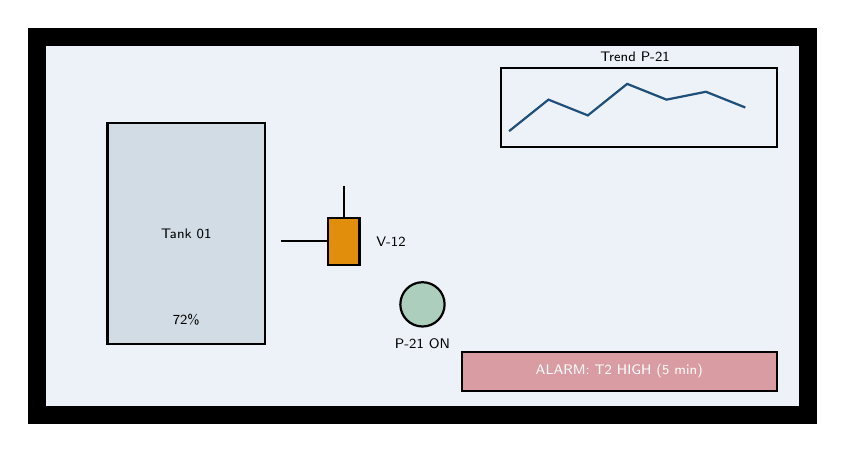
\begin{tikzpicture}
  \draw[thick, fill=black] (0,0) rectangle (10,5);
  \draw[thick, fill=isLight] (0.2,0.2) rectangle (9.8,4.8);
  % tank
  \draw[thick, fill=isOT!20] (1,1) rectangle (3,3.8);
  \node[font=\tiny] at (2,2.4) {Tank 01};
  \node[font=\tiny] at (2,1.3) {72\%};
  % valve
  \draw[thick] (3.2,2.3) -- (4,2.3) -- (4,3);
  \draw[thick, fill=isAccent] (3.8,2) rectangle (4.2,2.6);
  \node[font=\tiny] at (4.6,2.3) {V-12};
  % pump
  \draw[thick, fill=isHMI!40] (5,1.5) circle (8pt);
  \node[font=\tiny] at (5,1) {P-21 ON};
  % trend
  \draw[thick] (6,3.5) rectangle (9.5,4.5);
  \draw[thick, isOT] (6.1,3.7) -- (6.6,4.1) -- (7.1,3.9) -- (7.6,4.3) -- (8.1,4.1) -- (8.6,4.2) -- (9.1,4.0);
  \node[font=\tiny] at (7.7,4.65) {Trend P-21};
  % alarm bar
  \draw[thick, fill=isAttack!50] (5.5,0.4) rectangle (9.5,0.9);
  \node[font=\tiny, white] at (7.5,0.65) {ALARM: T2 HIGH (5 min)};
\end{tikzpicture}
\par\vspace{2mm}
{\footnotesize Mimic diagrams, trends, alarm bars. Bad HMI design $=$ accidents (Three Mile Island, 1979).}
\end{frame}

\begin{frame}{Historian -- Time-Series of the Plant}
\centering
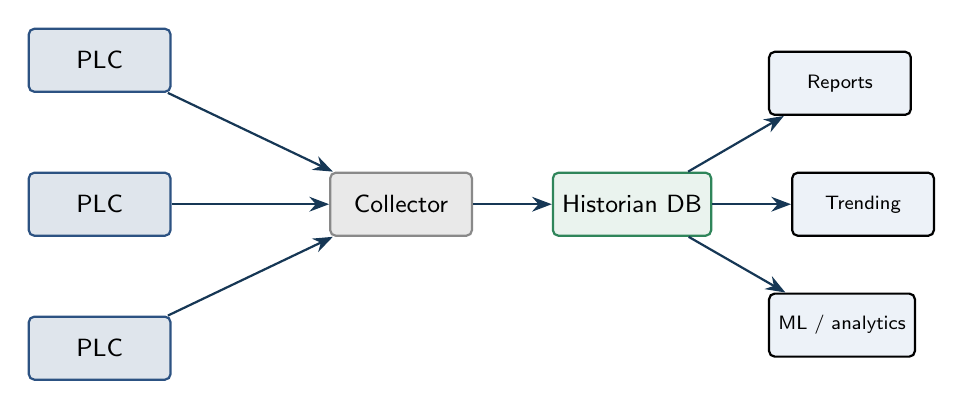
\begin{tikzpicture}[node distance=10mm]
  \node[plc] (p1) {PLC};
  \node[plc, below=of p1] (p2) {PLC};
  \node[plc, below=of p2] (p3) {PLC};
  \node[server, right=20mm of p2] (coll) {Collector};
  \node[server, right=of coll, fill=isHMI!10, draw=isHMI] (hist) {Historian DB};
  \node[isbox, above right=of hist, font=\scriptsize] (rep) {Reports};
  \node[isbox, right=of hist, font=\scriptsize] (trend) {Trending};
  \node[isbox, below right=of hist, font=\scriptsize] (ml) {ML / analytics};
  \foreach \p in {p1,p2,p3}{\draw[flow] (\p) -- (coll);}
  \draw[flow] (coll) -- (hist);
  \foreach \n in {rep,trend,ml}{\draw[flow] (hist) -- (\n);}
\end{tikzpicture}
\par\vspace{1mm}
{\footnotesize Historians bridge OT and IT; a frequent pivot point for attackers.}
\end{frame}

\section{Safety Layer}

\begin{frame}{Safety Instrumented Systems (SIS)}
\centering
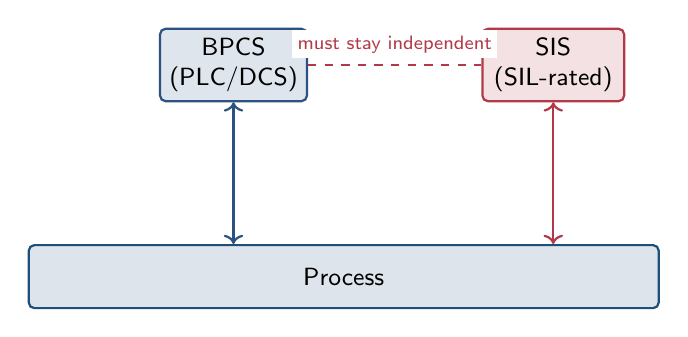
\begin{tikzpicture}[node distance=14mm]
  \node[plc, fill=isPLC!15, align=center] (bpcs) {BPCS\\(PLC/DCS)};
  \node[plc, fill=isAttack!15, draw=isAttack, align=center, right=22mm of bpcs] (sis) {SIS\\(SIL-rated)};
  \node[process, minimum width=80mm, below=18mm of bpcs.south, xshift=14mm] (proc) {Process};
  \draw[<->, thick, isPLC] (bpcs.south) -- (bpcs.south |- proc.north);
  \draw[<->, thick, isAttack] (sis.south) -- (sis.south |- proc.north);
  \draw[dashed, isAttack, thick] (bpcs.east) -- node[above=2pt, font=\scriptsize, isAttack, fill=white, inner sep=2pt]{must stay independent} (sis.west);
\end{tikzpicture}
\vspace{2mm}
\begin{notebox}{Safety layer}
The SIS brings the process to a safe state on demand. \textbf{IEC 61511 / 61508}, SIL 1--4.
\end{notebox}
\source{IEC 61508 (2010, ed.\,2.0), IEC 61511 (2016--17, ed.\,2.0) \textbar{} TRITON: Dragos \emph{TRISIS Malware Analysis}, 2017.}
\end{frame}

\begin{frame}{IEC 61131-3 -- PLC Programming Languages}
\centering
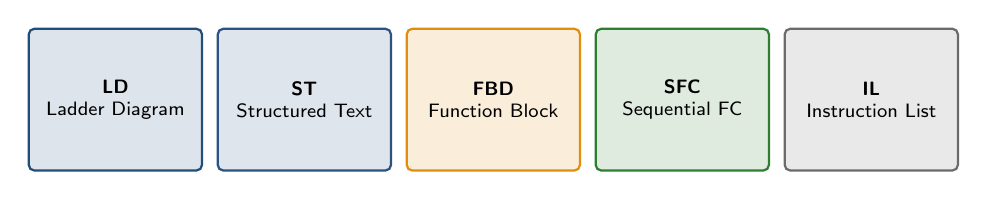
\begin{tikzpicture}[x=2.4cm]
  \foreach \i/\code/\name/\col in {
    0/LD/{Ladder Diagram}/isOT,
    1/ST/{Structured Text}/isPLC,
    2/FBD/{Function Block}/isAccent,
    3/SFC/{Sequential FC}/isNet,
    4/IL/{Instruction List}/isMute}{
    \node[isbox, fill=\col!15, draw=\col, font=\scriptsize, minimum width=22mm, minimum height=18mm, align=center] at (\i,0)
      {\textbf{\code}\\\name};
  }
\end{tikzpicture}
\vspace{2mm}
\begin{notebox}{The big two in the wild}
LD dominates discrete manufacturing; ST is the cross-vendor portable choice for new development.
\end{notebox}
\end{frame}

\begin{frame}{Engineering Workstation -- High-Value Target}
\centering
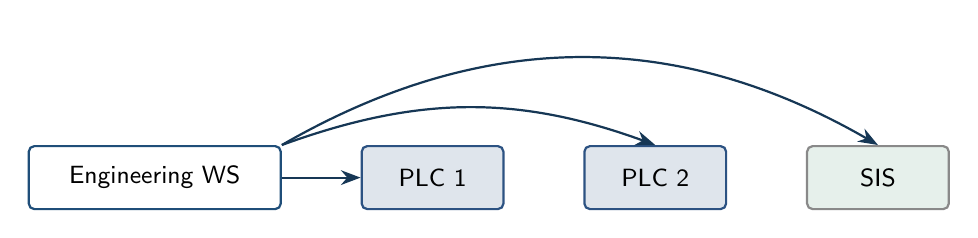
\begin{tikzpicture}[node distance=10mm]
  \node[workstation, minimum width=32mm] (ws) {Engineering WS};
  \node[plc, right=of ws] (p1) {PLC 1};
  \node[plc, right=of p1] (p2) {PLC 2};
  \node[server, right=of p2, fill=isHMI!12] (sis) {SIS};
  \draw[flow] (ws.east) -- (p1.west);
  \draw[flow] (ws.north east) to[bend left=20] (p2.north);
  \draw[flow] (ws.north east) to[bend left=30] (sis.north);
\end{tikzpicture}
\vspace{2mm}
\begin{warnbox}{Why attackers love it}
The engineering WS holds the credentials, project files, and the ability to \emph{re-flash logic}. Treat it as the crown jewel of the plant.
\end{warnbox}
\end{frame}

\begin{frame}{Process Types -- Batch, Continuous, Discrete}
\centering
\renewcommand{\arraystretch}{1.3}
\footnotesize
\begin{tabular}{|p{3cm}|p{3.5cm}|p{5cm}|}
\hline
\rowcolor{slidePanel}
\textbf{Type} & \textbf{Examples} & \textbf{Control system flavour} \\
\hline
Continuous & Refinery, power, water & DCS, tight feedback control \\
Batch      & Pharma, food, chemicals & DCS + recipe management (ISA-88) \\
Discrete   & Auto assembly, packaging & PLCs, fast cycle, ladder logic \\
\hline
\end{tabular}
\vspace{2mm}
\begin{notebox}{Why this matters for security}
Different processes have different ``safe states'' -- shutdown is fine for discrete, may be catastrophic for continuous. IR plans must reflect that.
\end{notebox}
\end{frame}

\begin{frame}{Summary -- Section \sectionNumber}
\begin{takeawaybox}{What to remember from this section}
\begin{itemize}\setlength{\itemsep}{2pt}
  \item Control loops close from sensors through PLC/DCS to actuators.
  \item SCADA aggregates field data; HMIs deliver situational awareness.
  \item Historians are the long-term memory and a common IT/OT bridge.
  \item SIS must remain independent --- attacking it was TRITON's goal in 2017.
\end{itemize}
\end{takeawaybox}
\end{frame}

\referencesframe{
  \item IEC 61131-3:2013. \emph{Programmable controllers -- Part 3: Programming languages}.
  \item IEC 61508 (ed.\,2.0, 2010). \emph{Functional safety of E/E/PE safety-related systems}.
  \item IEC 61511 (ed.\,2.0, 2016/17). \emph{Functional safety -- SIS for the process industry sector}.
  \item Morley, D. \emph{The history of the PLC}. Modicon, 2003 (interview/archive).
  \item Dragos. \emph{TRISIS Malware Analysis of Safety System Targeted Malware}, Dec 2017.
  \item ISA. \emph{ISA-101 Human Machine Interfaces for Process Automation Systems}, 2015.
  \item ISA-88. \emph{Batch Control Standards}.
  \item Krutz, R.L. \emph{Securing SCADA Systems}, Wiley, 2006.
  \item Macaulay, T., Singer, B. \emph{Cybersecurity for Industrial Control Systems}, CRC Press, 2012.
}

\closingframe

\end{document}
